%% ACM MM 2026 Submission - SGDAgent
%% Based on sample-sigconf.tex from acmart package
%
%% Commands for TeXCount
%TC:macro \cite [option:text,text]
%TC:macro \citep [option:text,text]
%TC:macro \citet [option:text,text]
%TC:envir table 0 1
%TC:envir table* 0 1
%TC:envir tabular [ignore] word
%TC:envir displaymath 0 word
%TC:envir math 0 word
%TC:envir comment 0 0
%%

\documentclass[sigconf, screen, review, anonymous]{acmart}
%%\documentclass[UTF8]{ctexart}
\AtBeginDocument{
  \providecommand\BibTeX{{Bib\TeX}}}

%% Rights management information
\setcopyright{acmlicensed}
\copyrightyear{2026}
\acmYear{2026}
\acmDOI{XXXXXXX.XXXXXXX}

%% Conference information
\acmConference[ACM MM '26]{ACM Multimedia 2026}{October 2026}{Rio de Janeiro, Brazil}
\acmISBN{978-1-4503-XXXX-X/2026/10}

%% Uncomment and fill if you have a submission ID from OpenReview
%%\acmSubmissionID{123-A56-BU3}

%% Additional packages
\usepackage{algorithm}
\usepackage{algpseudocode}
\usepackage{amsmath}
\usepackage{multirow}
\usepackage{graphicx}
\begin{document}

%%
%% Title
%%
\title{Scene Graph Database Agent: Hierarchical Spatio-Temporal Scene Graph Driven Agent for Long Video Understanding}

%%
%% Authors (hidden in anonymous mode)
%%
\author{Anonymous Author(s)}
\affiliation{%
  \institution{Anonymous Institution}
  \country{Anonymous}}

\renewcommand{\shortauthors}{Anonymous}

%%
%% Abstract
%%
\begin{abstract}

Long-form video understanding requires locating specific evidence—\ often involving particular entities, their relations, and precise temporal context—across videos that may span hours. 
Recent agentic approaches build a searchable caption database and let a reasoning model iteratively query it; yet captions are flat text without entity or temporal structure, 
causing semantic drift, redundant searches, and frequent failure to converge.
We propose SGDAgent, which augments the caption database with a hierarchical spatio-temporal scene graph index to convert open-ended search into structured candidate verification. 
The index comprises three levels—frame-level entity–relation graphs capturing spatial snapshots, segment-level temporal interaction graphs aggregating entity dynamics within sliding windows, 
and a global event graph encoding cross-segment event chains—all linked by a 
unified entity registry for cross-scale identity consistency. On this index, a graph-driven reasoning agent follows a propose–verify–answer paradigm: graph queries propose 
spatiotemporally grounded candidate windows, frame-level visual inspection verifies candidates on raw frames, and an uncertainty-aware control layer governs evidence sufficiency and fallback.
Under strictly matched settings on LVBench (same backbone, caption source, and budget), SGDAgent raises end-to-end accuracy from 54.8\% to 73.0\% and reduces the failed-termination rate from 
16.5\% to 1.6\% over the caption-only baseline. Trajectory analysis confirms that the gains stem from restructuring the search process—shifting from open retrieval to graph-anchored candidate 
verification—rather than from the graph directly producing answers.
\end{abstract}

%%
%% CCS Concepts - Generate yours at https://dl.acm.org/ccs
%%
\begin{CCSXML}
<ccs2012>
 <concept>
  <concept_id>10010147.10010178.10010224</concept_id>
  <concept_desc>Computing methodologies~Computer vision</concept_desc>
  <concept_significance>500</concept_significance>
 </concept>
 <concept>
  <concept_id>10010147.10010257.10010293.10010294</concept_id>
  <concept_desc>Computing methodologies~Neural networks</concept_desc>
  <concept_significance>300</concept_significance>
 </concept>
 <concept>
  <concept_id>10002951.10003317.10003347.10003352</concept_id>
  <concept_desc>Information systems~Question answering</concept_desc>
  <concept_significance>500</concept_significance>
 </concept>
</ccs2012>
\end{CCSXML}

\ccsdesc[500]{Computing methodologies~Computer vision}
\ccsdesc[300]{Computing methodologies~Neural networks}
\ccsdesc[500]{Information systems~Question answering}

%%
%% Keywords
%%
\keywords{long-form video question answering, scene graph, agentic reasoning, multimodal retrieval, candidate verification}

\maketitle

%%
%% ==================== BODY ====================
%%

\section{Introduction}
\label{sec:intro}

% ---- Para 1: Background → agentic search → core problem ----

Answering questions about long-form videos requires locating specific
evidence---often involving particular entities, their relations, and
precise temporal context---within a timeline that may span hours.  Recent
agentic approaches convert the video into a searchable caption database
and let a reasoning LLM iteratively query
it~\cite{dvd,videoagent,videoseek}; yet \emph{the search space is
unstructured}: captions are flat text without entity identities, relation
bindings, or temporal anchoring, easily causing semantic drift, redundant
searches, and trajectories that fail to converge.

% ---- Para 2: Prior efforts share the same limitation ----

Recent works have begun to address this instability by improving the
agent's search strategy---through multi-round frame
retrieval~\cite{videoagent}, explicit grounding--verification
pipelines~\cite{videomind}, or multi-granularity
toolkits~\cite{videoseek}---yet they all leave the underlying evidence
space essentially unchanged: flat captions or raw frames.  A common thread
is that these methods improve \emph{how the agent searches} without
restructuring \emph{what it searches over}.  This raises a natural
question: can the evidence space itself be reorganized to yield more
stable and verifiable search trajectories?

% ---- Para 3: Scene graphs → spatio-temporal gap → our opportunity ----

Scene graphs---structured representations that bind entities, attributes,
and pairwise relations---offer a natural candidate for such
reorganization, as they provide exactly the entity-level and relational
grounding that flat captions lack~\cite{scenegraph1,scenegraph2}. Recent
video scene graph generation methods further extend this idea to
temporally evolving visual relations across frames~\cite{tpt}.
However, two gaps prevent
their direct application to long-form video QA\@.  First, a single-frame
scene graph captures only a \emph{spatial} snapshot and cannot represent
temporal interactions or cross-segment entity continuity across an extended
timeline.  Second, no prior work has built a reasoning agent that uses
scene graphs as its \emph{primary retrieval index}---one that queries
graph structure to propose candidates and verifies them visually, rather
than treating graphs as a post-hoc annotation.

% ---- Para 4: Our method — representation + agent workflow ----

We propose \textbf{SGDAgent}, which addresses both gaps.  On the
representation side, we construct a \emph{hierarchical spatio-temporal
scene graph index} that augments the caption database with three levels of
structured knowledge: frame-level entity--relation graphs that capture
per-keyframe spatial snapshots, segment-level temporal interaction graphs
that aggregate entity dynamics within sliding windows, and a global event
graph that encodes cross-segment event chains with explicit temporal and
semantic edges.  A shared video-level entity registry links all three levels
to maintain identity consistency across scales.  On the reasoning side, we
build a graph-driven agent that operates in an observe--reason--act loop
over this augmented database.  At each reasoning step the agent can invoke
graph queries at any level to \emph{propose} a small set of
spatiotemporally grounded candidate windows, then call frame-level visual
inspection to \emph{verify} candidates on raw frames, with caption search
serving as a complementary fallback channel.  An uncertainty-aware control
layer---comprising query-type routing, confidence gating, and terminal
convergence---governs when accumulated evidence is sufficient to commit an
answer.  This design converts the agent's core search process from
open-ended caption retrieval into structured candidate verification: the
graph narrows \emph{where to look}, visual inspection confirms \emph{what
is there}, and the control layer ensures the trajectory converges
reliably.

% ---- Para 5: Results ----

Under strictly matched settings on LVBench~\cite{lvbench} (same backbone,
caption source, and budget), SGDAgent raises end-to-end accuracy from
54.8\% to 73.0\% and reduces the failed-to-terminate (FTT) rate from
16.5\% to 1.6\% compared with the caption-only baseline.  Across four
benchmarks, SGDAgent with the lighter \texttt{o4-mini} backbone
consistently approaches or matches DVD with the substantially stronger
\texttt{o3}, suggesting that the structured graph index compensates for
weaker open-ended search capability.  Ablation and trajectory analyses
confirm that the improvement stems from restructuring the search process
itself---shifting from open retrieval to graph-anchored candidate
verification---rather than from the graph directly producing answers.

% ---- Para 6: Contributions ----

Our main contributions are:
\begin{itemize}
\item A \textbf{hierarchical spatio-temporal scene graph index} for long
  videos, comprising frame-level, segment-level, and global event-level
  graphs linked by a shared entity registry, together with a bottom-up
  construction pipeline that builds all three levels offline from
  VLM-extracted keyframe graphs.

\item A \textbf{graph-driven reasoning agent} that follows a
  propose--verify--answer paradigm within an observe--reason--act loop,
  with graph-guided candidate proposal, frame-level visual verification,
  caption-based fallback, and uncertainty-aware control strategies that
  convert open-ended search into structured candidate verification.

\item \textbf{Comprehensive evaluation} on four long-video benchmarks
  (LVBench, LongVideoBench, Video-MME, and Ego\-Schema), with strictly
  matched ablation and behavioral analyses on LVBench confirming that the
  gains stem from restructuring the search paradigm rather than the graph
  directly producing answers.
\end{itemize}

\section{Related Work}
\label{sec:related}
 
\textbf{Long-video understanding.}\quad
Existing methods fall into two broad classes.  The first extends context
capacity or compresses visual redundancy through longer context
windows, token compression, or hierarchical video
representations~\cite{gemini15,qwen,internvl,seed}; these improve input
coverage but still must locate sparse, question-relevant evidence within
compressed representations.  The second treats long-video understanding as
a retrieval or search problem, progressively mining relevant information
through selective sampling, external databases, or agentic
search~\cite{dvd,mrvideo,videoseek}.  SGDAgent belongs to the second
class but differs in focus: rather than performing stronger query
reformulation over the caption database alone, we ask whether the
\emph{evidence space itself} can be restructured---extending the caption
database with a structured scene graph index so that the main retrieval
steps become candidate proposal processes grounded in entities, relations,
and temporal constraints.
 
\textbf{Agentic video reasoning.}\quad
A growing body of work models long-video understanding as an agentic
reasoning problem.  VideoAgent~\cite{videoagent} controls multi-round
frame retrieval and self-reflection through an LLM-driven
state--action--observation loop.  DVD~\cite{dvd} establishes agentic
search over a multi-granularity video database, letting the LLM
adaptively invoke tools at different temporal scales.
VideoSeek~\cite{videoseek} designs a multi-granularity toolkit that
mirrors human seeking behavior.  These methods progressively improve the
flexibility and efficiency of the agent's search strategy, yet they all
operate over the same evidence space---flat captions or raw frames.
SGDAgent extends the agent's action space from caption retrieval to a
cascaded process of graph-guided candidate proposal, visual verification,
and controlled fallback, thereby transforming the core search space from
an open-ended caption space to a graph-anchored candidate space.
 
\textbf{Temporal grounding and verification.}\quad
VideoMind~\cite{videomind} argues that effective video reasoning requires
a phased process of moment localization, boundary verification, and
answer generation, implementing this through four specialized roles
(Planner, Grounder, Verifier, Answerer) on a unified backbone.  SGDAgent
shares the view that long-form video QA benefits from a phased
\emph{localize--verify--answer} process, but differs in mechanism: rather
than training a dedicated grounding backbone, we use multi-level scene
graphs to progressively propose candidates at event, segment, and frame
granularities, then delegate final confirmation to visual inspection.
Grounding is thus jointly accomplished by the structured graph index and
online agent strategy rather than solely by a learned module.
 
\section{Methodology}
\label{sec:method}

% --- SGDAgent overview ---
SGDAgent augments the caption database with a \emph{hierarchical
spatio-temporal scene graph index} that converts open-ended caption search
into graph-anchored candidate verification.  As illustrated in
Figure~\ref{fig:mechanism}, the system consists of three components.
%
\textbf{(i)~Hierarchical scene graph representation}
(Section~\ref{sec:representation}): a three-level structured index
comprising frame-level graphs $G^{f}$, segment-level graphs $G^{s}$, and a
global event graph $G^{g}$, which together with the caption database
$C(V)$ form an augmented video database
$D(V)=\{C(V),\;G^{f},\;G^{s},\;G^{g}\}$.
%
\textbf{(ii)~Offline graph construction}
(Section~\ref{sec:construction}): a bottom-up pipeline that extracts
frame-level entity--relation graphs via a VLM, merges them into
segment-level temporal graphs through sliding-window aggregation, and
further clusters segments into a global event graph with explicit event
edges.
%
\textbf{(iii)~Graph-driven agent} (Section~\ref{sec:agent}): an online
reasoning agent that operates in an observe--reason--act loop over the
augmented database, following a \emph{propose--verify--answer}
paradigm---graph queries propose spatiotemporally grounded candidate
windows, frame-level visual inspection verifies candidates on raw frames,
and an uncertainty-aware controller governs evidence sufficiency and
fallback.
%
Algorithm~\ref{alg:search} summarizes the online search procedure.

\begin{figure*}[t]
    \centering
    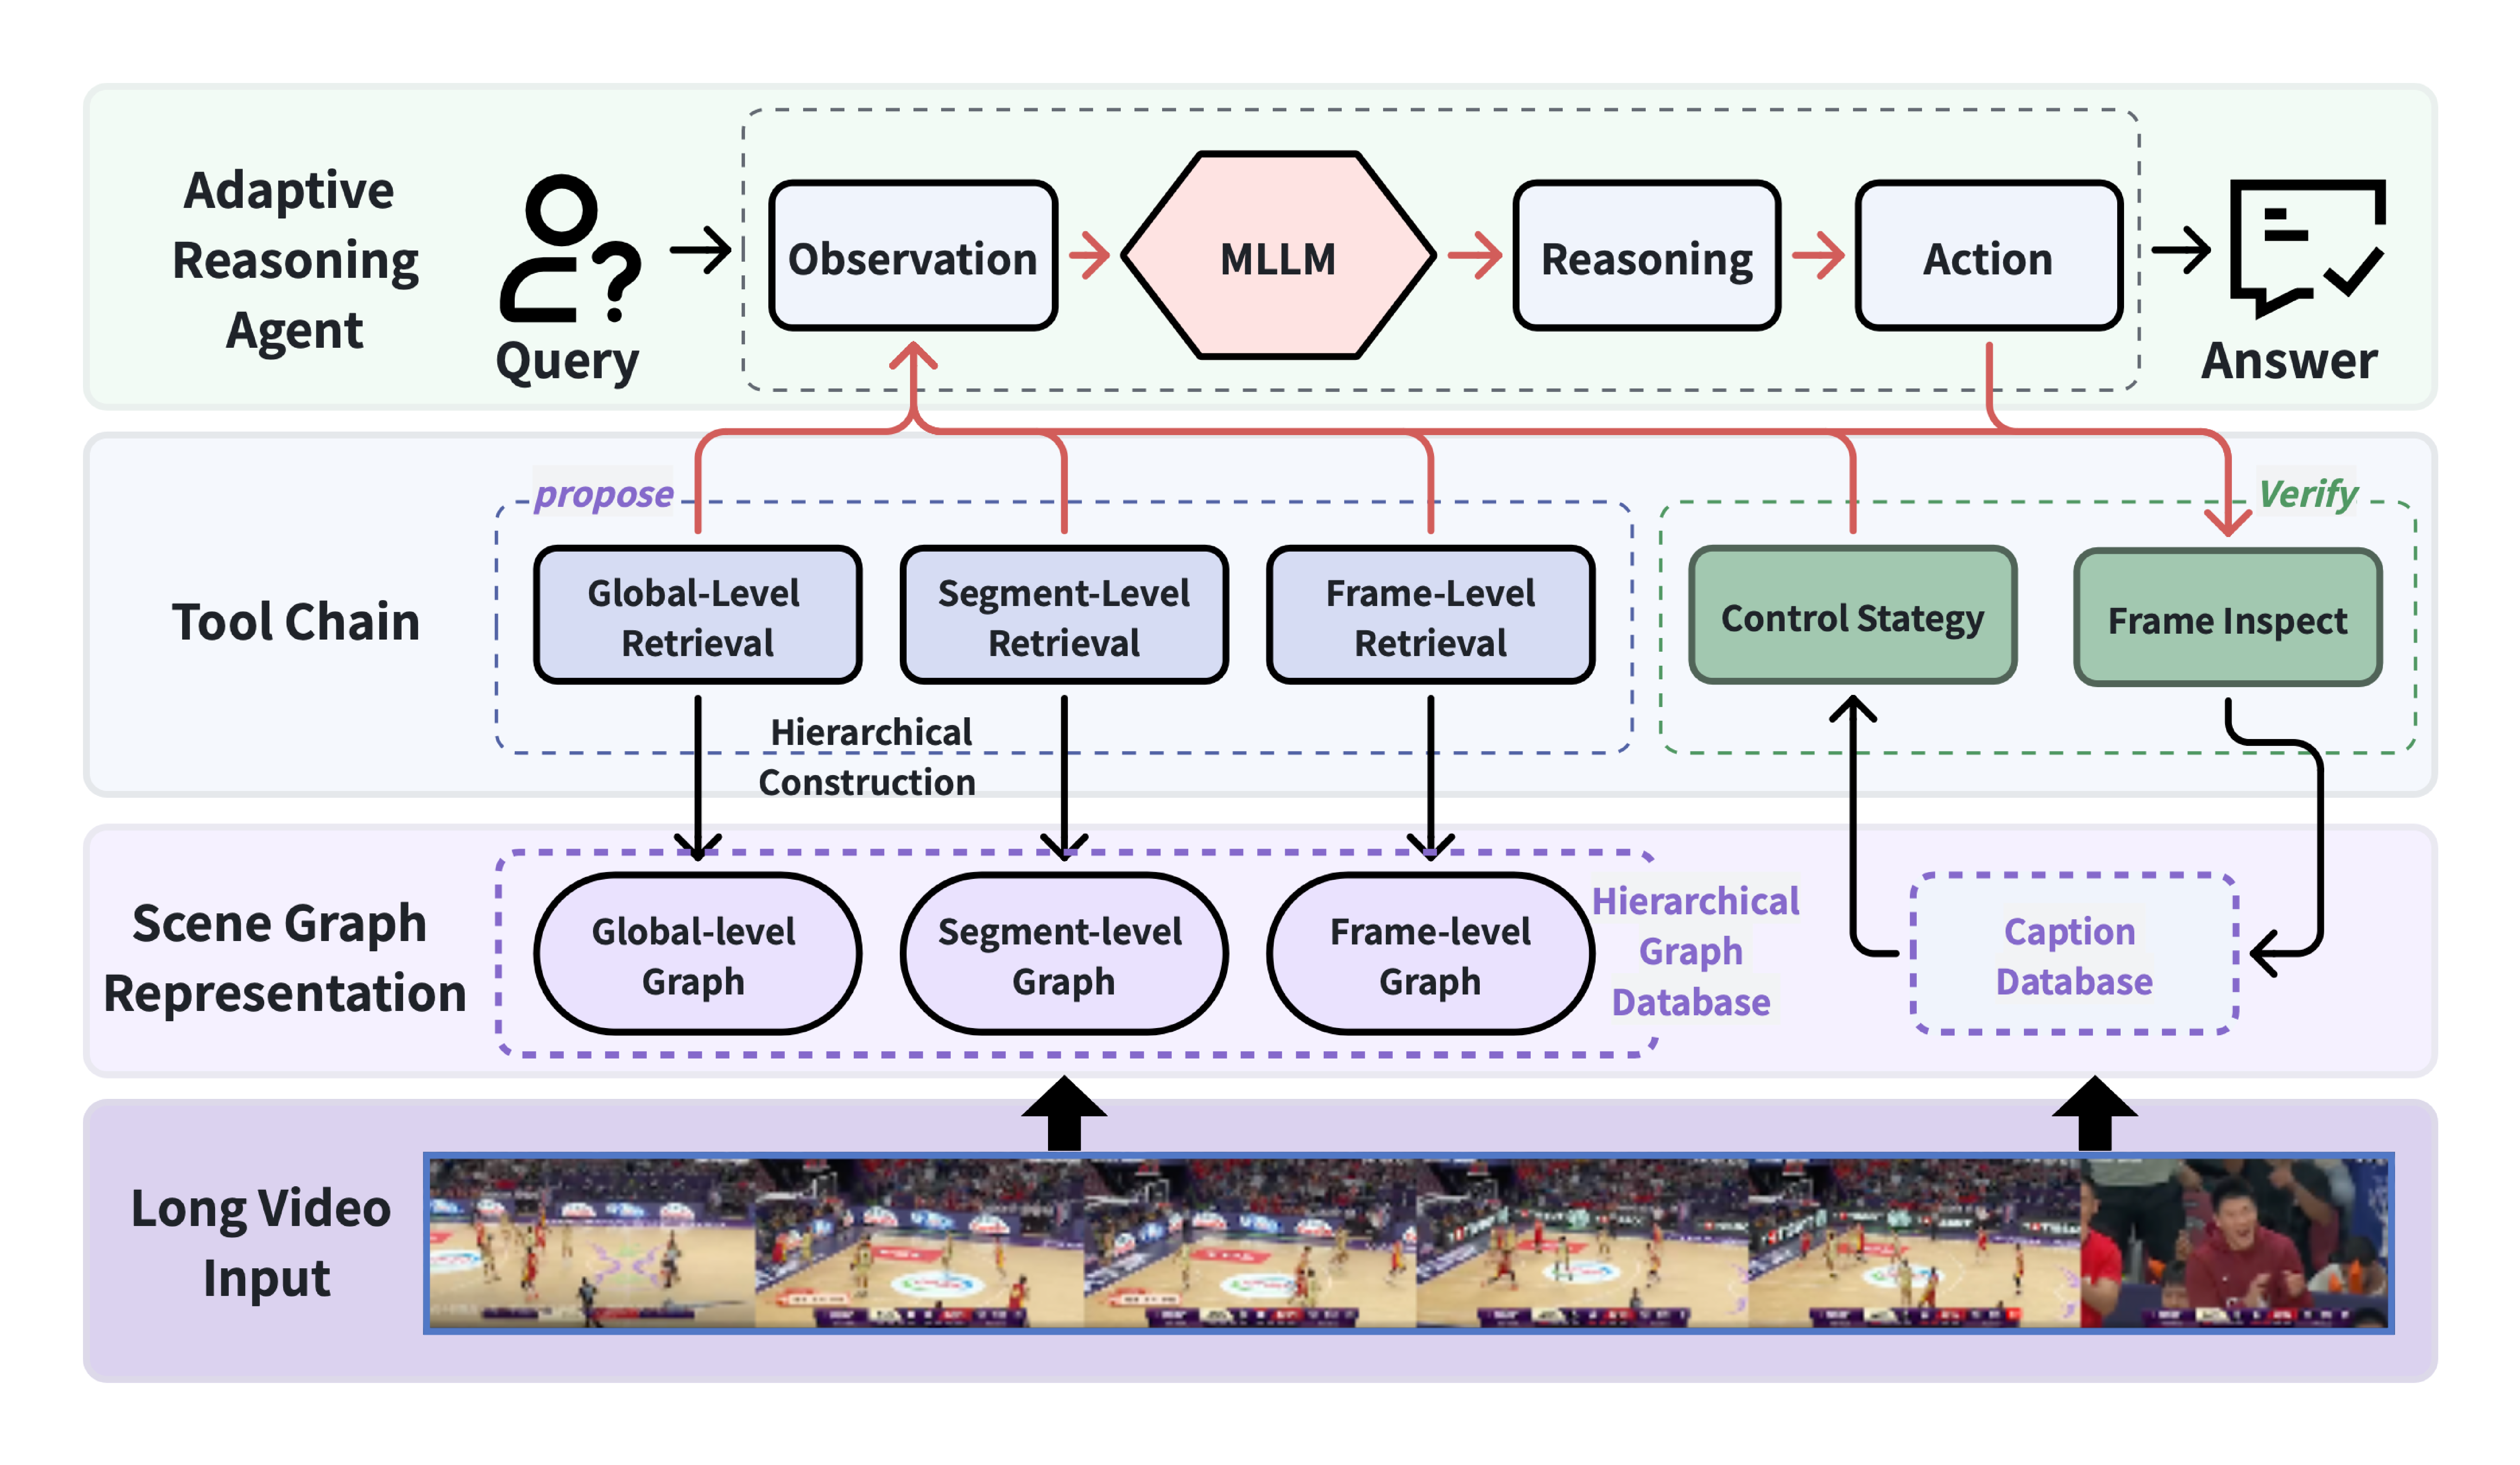
\includegraphics[width=0.85\textwidth]{figures/workflow.pdf}
    \caption{Overview of SGDAgent. Long videos are converted into a
    scene-graph-augmented video database with global-, segment-, and
    frame-level graphs plus a caption database. An adaptive reasoning
    agent then searches this database through a propose--verify tool
    chain within an observe--reason--act loop.}
    \label{fig:mechanism}
\end{figure*}

\begin{algorithm}[t]
\caption{Graph-Guided Search}
\label{alg:search}
\begin{algorithmic}[1]
\Require Augmented database $D(V)=\{C(V), G^f, G^s, G^g\}$, question $q$
\Ensure Answer $\hat{a}$
\State Parse $q$ into structural constraints $\phi(q)$
  and routing type $\pi(q)$
\If{$q$ involves long-range temporal or event-level cues}
    \State Propose event candidates on $G^g$;
      cascade to supporting segments on $G^s$
\Else
    \State Propose candidate windows directly on $G^s$
\EndIf
\Repeat
    \If{fine-grained object anchoring is needed}
        \State Refine candidates on $G^f$
    \EndIf
    \State $Z_q \leftarrow$ verify top candidates via
      \texttt{frame\_inspect} on raw frames
    \If{gating conditions satisfied}
        \State \Return $\mathrm{Answer}(q, Z_q)$
    \ElsIf{graph evidence weak or stagnation detected}
        \State Fall back to caption search or global browse
    \EndIf
\Until{answer committed or budget exhausted}
\State Force terminal convergence from accumulated evidence
\end{algorithmic}
\end{algorithm}


% ==================================================================
%  3.1  Hierarchical Scene Graph Representation
% ==================================================================
\subsection{Hierarchical Scene Graph Representation}
\label{sec:representation}

SGDAgent organizes video-level knowledge as the caption database augmented
with a three-level spatio-temporal scene graph index
(Figure~\ref{fig:graph}):
\begin{equation}
  D(V) = \bigl\{C(V),\; G^{f},\; G^{s},\; G^{g}\bigr\},
\end{equation}
where $C(V)$ is the caption database inherited from DVD for open semantic
retrieval; $G^{f}=\{G_i^{f}\}_{i=1}^{N}$ is the frame-level graph
sequence; $G^{s}=\{G_j^{s}\}_{j=1}^{M}$ is the segment-level graph
sequence; and $G^{g}=(V^{g},\,\mathcal{E}^{g})$ is the global event graph,
with event node set $V^{g}$ and event edge set $\mathcal{E}^{g}$.
All three graph levels share a video-level entity registry
$E^{\text{video}}$, where each entry stores a unique ID, entity type,
attributes, description, and temporal span (first and last appearance),
serving as the cross-scale identity anchor.

\begin{figure*}[t]
    \centering
    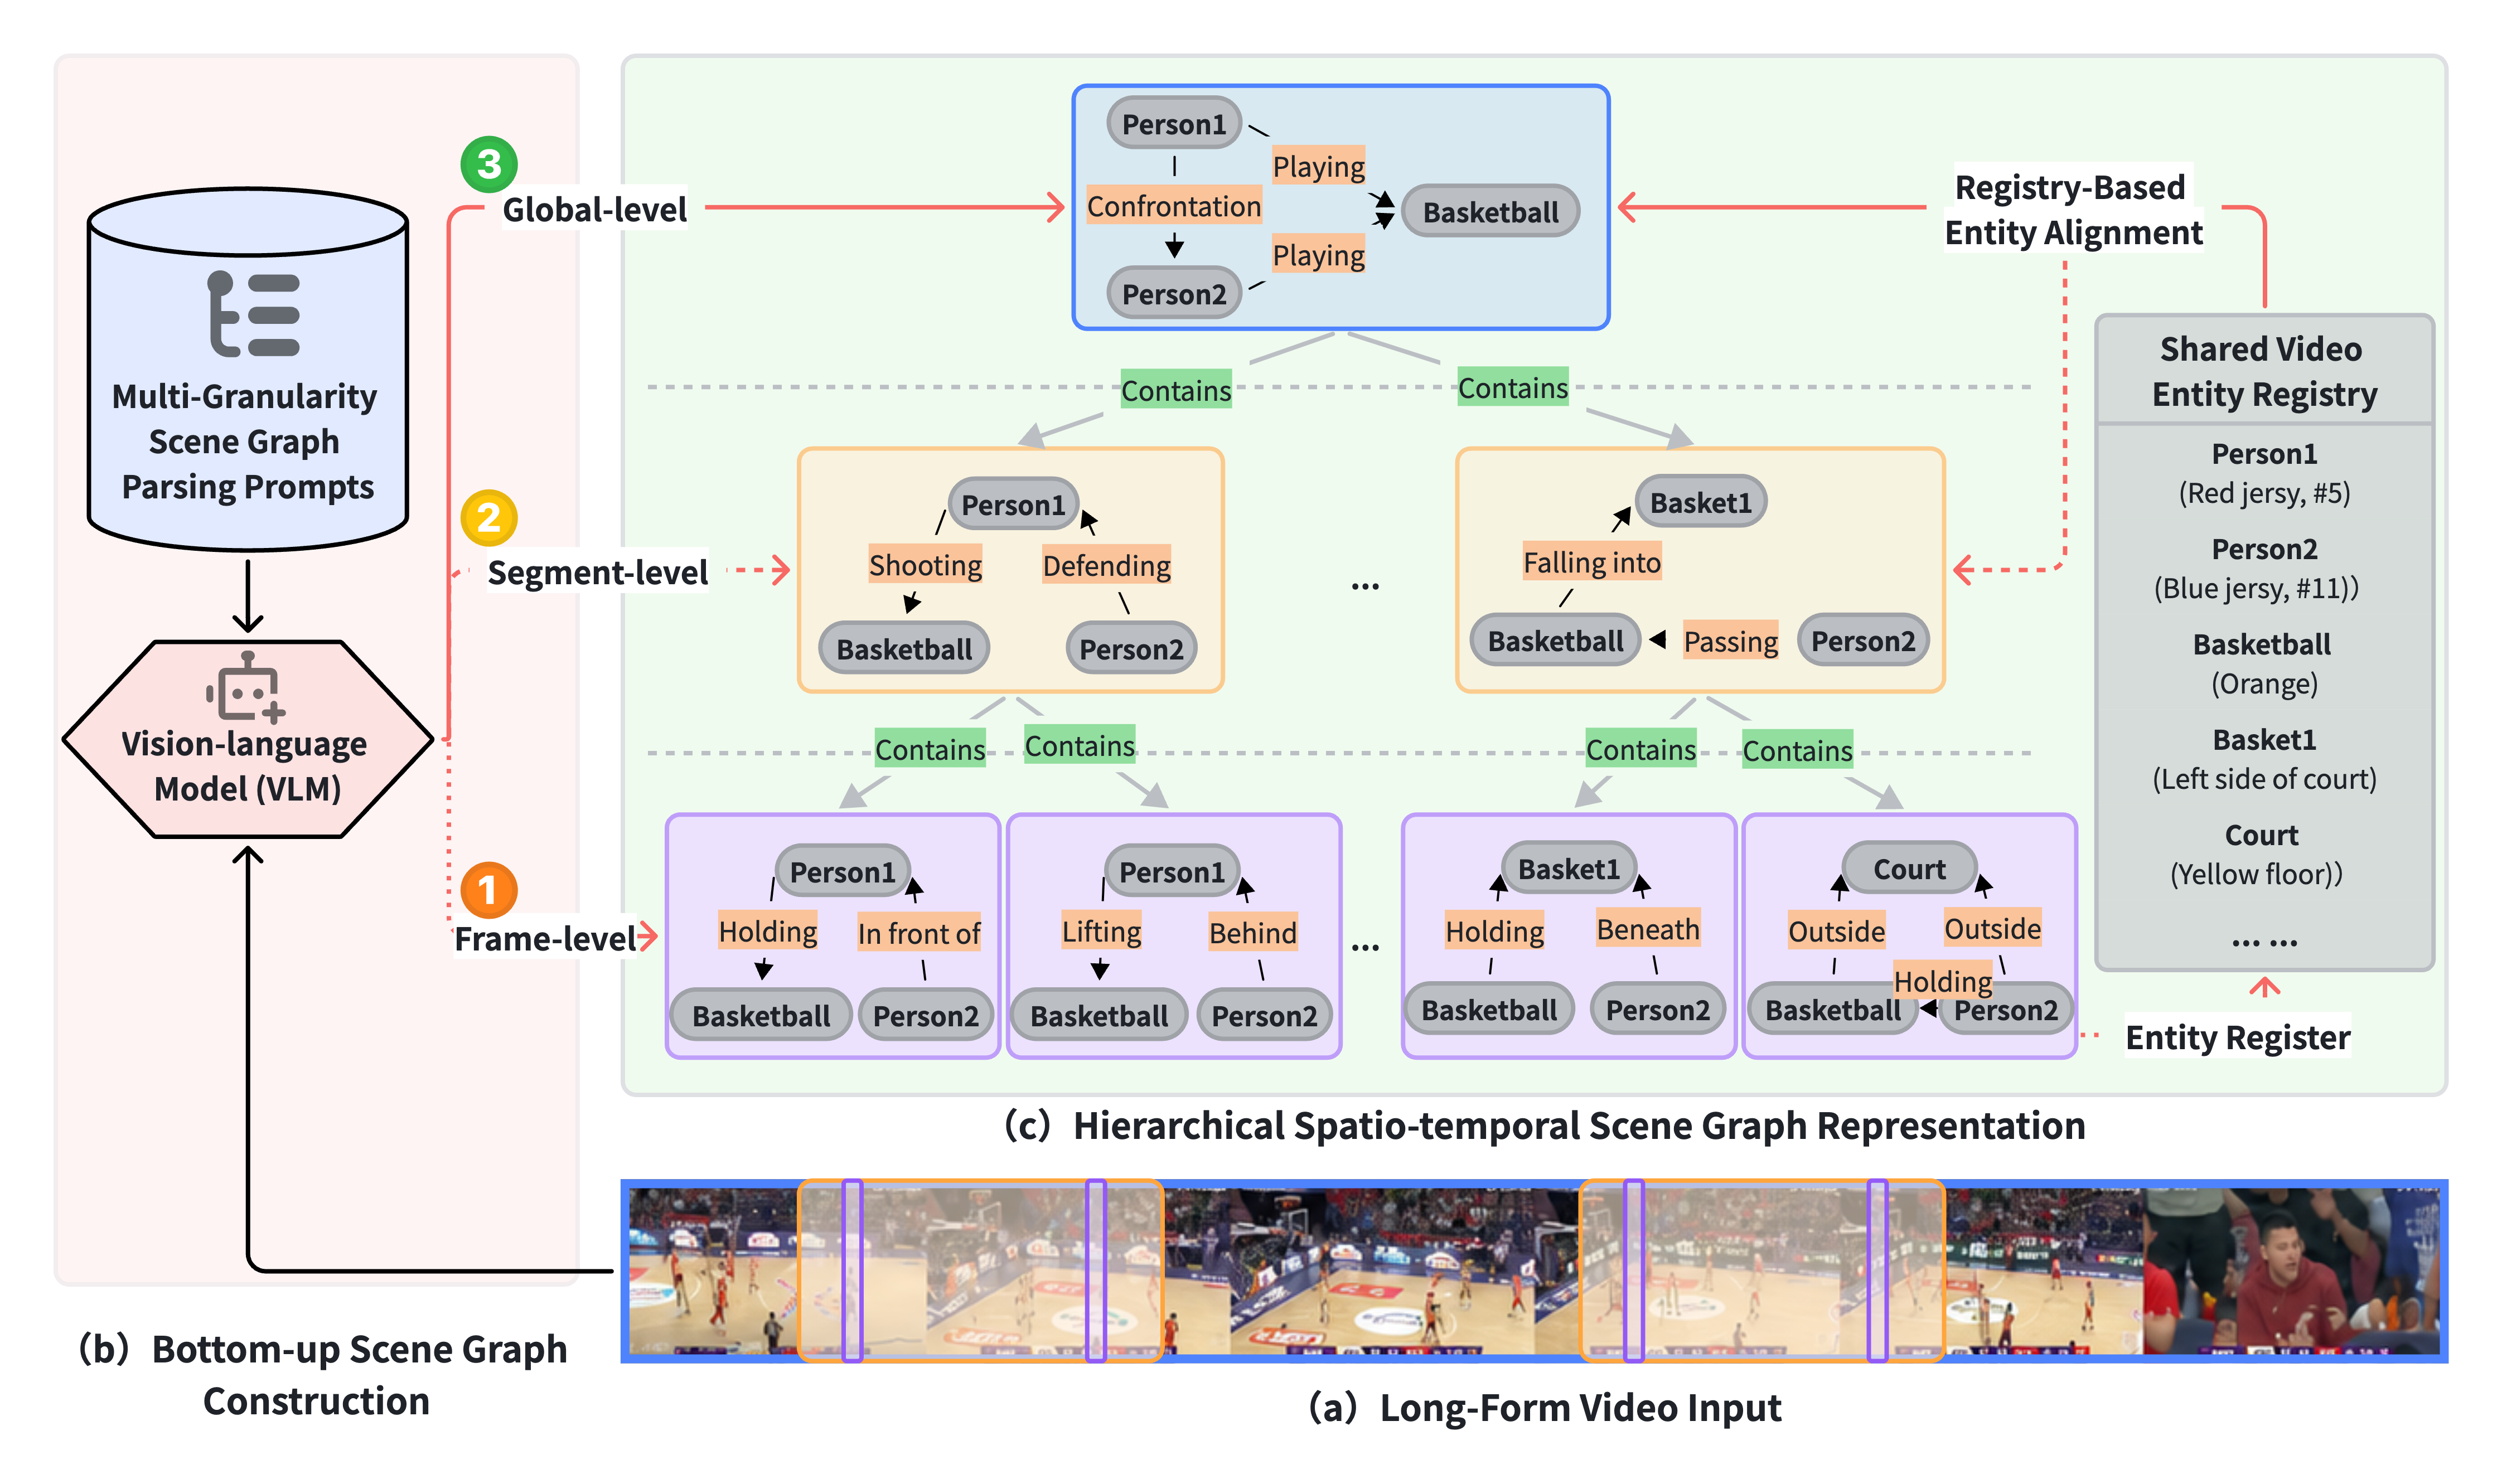
\includegraphics[width=0.85\textwidth]{figures/Graph.png}
    \caption{Hierarchical scene graph representation and bottom-up
    construction pipeline.  (a)~Keyframes are sampled from the long video.
    (b)~A VLM generates frame-level scene graphs; entity alignment
    maintains identity consistency via a shared video-level entity
    registry.  (c)~The three-level representation: frame-level graphs
    capture per-keyframe entity--relation snapshots, segment-level graphs
    aggregate temporal interactions within sliding windows, and the global
    event graph organizes high-level event semantics with explicit event
    edges.}
    \label{fig:graph}
\end{figure*}

\textbf{Frame-level graph.}\quad
Each frame-level graph captures the entity--relation snapshot at a single
keyframe:
\begin{equation}
  G_i^{f} = (E_i^{f},\; R_i^{f},\; t_i,\; c_i),
\end{equation}
where $E_i^{f} \subseteq E^{\text{video}}$ is the set of entities visible
in the frame, $R_i^{f}$ is the set of relation triples $(s, p, o)$ with
$s,o \in E_i^{f}$ and predicate $p$, $t_i$ is the timestamp, and $c_i$ is
the aligned caption context.  Frame-level graphs provide the finest spatial
granularity, anchoring individual objects and their local relations to
specific time points.

\textbf{Segment-level graph.}\quad
Each segment-level graph aggregates entity interactions over a short
temporal window:
\begin{equation}
  G_j^{s} = (E_j^{s},\; R_j^{s},\;
  [t_j^{\text{s}}, t_j^{\text{e}}],\; F_j,\; s_j),
\end{equation}
where $E_j^{s}$ is the active entity set within the segment, $R_j^{s}$ is
the set of temporal relations, $[t_j^{\text{s}}, t_j^{\text{e}}]$ is the
time range, $F_j$ is the set of supporting frame IDs, and $s_j$ is a
concise segment summary.  Each temporal relation is represented as
$(s, p, o, t_{\text{start}}, t_{\text{end}}, \mathcal{F})$, binding
participants to their temporal extent and supporting frames.

\textbf{Global event graph.}\quad
The global event graph $G^{g}=(V^{g},\,\mathcal{E}^{g})$ organizes
higher-level event semantics on top of segments.  Each event node
$n_k \in V^{g}$ is defined as
\begin{equation}
  n_k = (P_k,\; R_k,\;
  [t_k^{\text{s}}, t_k^{\text{e}}],\; S_k,\; F_k,\; \sigma_k),
\end{equation}
where $P_k$ is the participant entity set, $R_k$ is the salient relation
set, $[t_k^{\text{s}}, t_k^{\text{e}}]$ is the event time range, $S_k$ is
the set of supporting segment IDs, $F_k$ is the supporting frame set, and
$\sigma_k$ is the event summary.  Event nodes are typed as either
\emph{unit events} (compact local episodes) or \emph{group events}
(longer episodes composed of multiple units).  The event edge set
$\mathcal{E}^{g}$ contains typed edges---\texttt{before},
\texttt{overlaps}, \texttt{entity-carryover}, \texttt{same-thread}, and
\texttt{parent-child}---encoding cross-segment event chains and
hierarchical event structure.


% ==================================================================
%  3.2  Offline Graph Construction
% ==================================================================
\subsection{Hierarchical Scene Graph Construction}
\label{sec:construction}

The offline phase builds the three graph levels bottom-up---frame, then
segment, then global event---so that online reasoning can perform cascaded
retrieval over a pre-built structured index.

\textbf{Frame graph extraction and entity alignment.}\quad
Keyframes are uniformly sampled at a fixed interval.  For each keyframe, a
VLM produces a structured scene graph in a single pass, outputting typed
entities with attributes and relation triples.  Entity identity across
frames is maintained by greedily aligning each new entity to the
video-level registry $E^{\text{video}}$ via a weighted combination of name
similarity, description similarity, and type consistency; entities whose
score exceeds a threshold $\tau$ are merged, and the rest are registered as
new.  When the VLM fails to extract any entity, coarse-grained entities
are recovered from temporally neighboring captions to prevent empty-graph
gaps.

\textbf{Segment graph merging.}\quad
Frame-level graphs are aggregated into segment-level graphs using
overlapping sliding windows.  Within each window, frame-level relation
triples sharing the same $(s, p, o)$ signature are merged into a single
temporal relation whose extent spans the earliest to the latest supporting
frame; supporting frame IDs and occurrence counts are preserved.  Each
segment graph is equipped with a concise textual summary, and overlap links
between adjacent windows support cross-boundary retrieval.

\textbf{Event graph construction.}\quad
Temporally proximate and semantically coherent segments are clustered into
events.  Merging decisions are governed by temporal gap, shared entity
count, relation overlap, and predicate overlap; overly long or
discontinuous clusters are split into finer-grained unit events.  Group
events are formed from multiple units with \texttt{parent-child} edges.
Pairwise event edges---\texttt{before}, \texttt{overlaps},
\texttt{entity-carryover}, and \texttt{same\-thread}---are inferred from
temporal ordering and entity sharing, completing the event-level retrieval
graph.

\textbf{Quality control.}\quad
Throughout construction, lightweight constraints are applied: entity
blacklist filtering removes generic or uninformative entities, predicate
whitelist constraints suppress noisy relations, and schema validation
enforces structural consistency of each graph level.  At the event level,
confidence and uncertainty estimates are attached to each node to inform
downstream gating decisions.


% ==================================================================
%  3.3  Graph-Driven Agent
% ==================================================================
\subsection{Hierarchical Scene Graph Driven Agent}
\label{sec:agent}

\begin{sloppypar}
SGDAgent retains DVD's observe--reason--act backbone and its caption-based
tools (\texttt{clip\_search}, \texttt{global\_browse},
\texttt{frame\_inspect}) as fallback channels, while introducing graph
query tools at each level (\texttt{global\_graph\_query},
\texttt{segment\_graph\_query}, \texttt{frame\_graph\_query}) as the
primary candidate proposal interface.  The full tool set is
$\mathcal{T}=\{GG,\,SG,\,FG,\,FI,\,\textsc{Answer}\}$, where $GG$,
$SG$, $FG$ query the three graph levels and $FI$ performs visual
verification on raw frames.
\end{sloppypar}

\textbf{Reasoning loop.}\quad
At each reasoning step~$t$, the agent observes the current state---the
question, accumulated tool returns, reasoning history, and control
signals---and the backbone LLM selects the next action: querying a graph
level to propose candidates, invoking \texttt{frame\_inspect} to verify a
candidate window, falling back to caption search, or committing an answer.
Tool outputs are appended to the state for the next step, forming a closed
observe--reason--act loop (Algorithm~\ref{alg:search}).  Unlike pipeline
methods with a fixed workflow, the search path is driven jointly by the
question type, graph retrieval results, and runtime control signals,
allowing the agent to adaptively enter the graph hierarchy at any level
and drill down as needed.

\textbf{Proposal.}\quad
The system first extracts lightweight structural constraints from the
question---entity mentions, relation or action cues, temporal anchors, and
whether fine-grained visual attributes are involved---using rule-based
parsing.  These constraints drive a top-down cascade: for long-range
temporal or event-level questions, $GG$ retrieves matching events and
cascades their supporting segments to $SG$; for local relation or
short-range questions, candidates are proposed directly from $SG$; and when
object-level anchoring is needed, $FG$ further narrows candidates to
specific frames.  Candidates at each level are ranked by a composite score
\begin{equation}
  S(w \mid q) \;=\; S_{\text{lex}}(w,q) \;+\;
  S_{\text{soft}}(w,q) \;+\; S_{\text{temp}}(w,q),
\end{equation}
where $S_{\text{lex}}$ measures lexical match over entities, predicates,
and summaries, $S_{\text{soft}}$ captures embedding-based semantic
similarity, and $S_{\text{temp}}$ scores temporal consistency with
explicit time references or natural-language temporal anchors in $q$.

\textbf{Verification.}\quad
Graph-proposed candidates specify \emph{where to look} but do not
constitute terminal evidence.  For each top candidate window, the agent
invokes \texttt{frame\_inspect} to sample raw frames and perform visual
question answering conditioned on the query.  This two-stage separation
transforms frame inspection from a blind searcher over the entire video
into a focused verifier over graph-localized regions.

\textbf{Uncertainty-aware control.}\quad
Three lightweight mechanisms prevent premature commitment and indefinite
looping.  (1)~\emph{Query-type routing}: the question is classified into
routing types (summary, temporal chain, scene localization, fine detail,
other) that determine the initial graph level and the minimum evidence
requirements---e.g., fine-detail questions require narrow-window visual
inspection before an answer can be committed.  (2)~\emph{Confidence
gating}: when graph queries return weak or stagnating signals, the system
falls back to caption-based tools before resuming graph queries.
(3)~\emph{Terminal convergence}: when the budget is exhausted, a forced
procedure extracts the best-supported option from the accumulated trace,
preventing well-evidenced trajectories from being lost as FTT outcomes.
Section~\ref{sec:ablation} separately evaluates routing and gating versus
terminal convergence.

\section{Experiments}
\label{sec:experiments}


% ============================================================
%  Section 4.1  —  Experimental Setup
% ============================================================

\subsection{Experimental Setup}
\label{sec:setup}

\textbf{Dataset.}\quad
Our primary benchmark is \textbf{LVBench}~\cite{lvbench}, which contains
1{,}549 four-choice video QA questions over long-form videos.  The system
receives a video, a natural-language question, and four candidate answers,
and must return exactly one option; failure to do so is recorded as
a failed-to-terminate (FTT) outcome.

\textbf{Implementation details.}\quad
The reasoning backbone is \texttt{o4-mini} (temperature~0) with a maximum
of 15 reasoning steps per question.  Frame-level scene graphs (Stage~1)
are extracted by prompting \texttt{gpt-4.1} on keyframes sampled at one
frame every 5~seconds (up to 120 per video).  Segment-level graphs
(Stage~2) use 30-second sliding windows with 5-second overlap.  Local
visual verification is performed by \texttt{gpt-4.1-mini}, with a budget
of 50~frames per \texttt{frame\_inspect} call.  Graph retrieval returns at
most 5 event-level, 6 segment-level, and 8 frame-level candidates.  To
ensure fair matched-setting comparison, all internally compared methods
share the same reasoning backbone, frame-inspect VLM, caption source,
video database, candidate answer set, and budget limits; all methods are
permitted to produce FTT outcomes.

\textbf{Evaluation metrics.}\quad
We report four complementary metrics: \emph{end-to-end accuracy}
(e2e\_acc), the fraction of all questions answered correctly;
\emph{answered accuracy} (ans\_acc), accuracy computed only over questions
for which the system produced a valid option; \emph{answer rate}, the
fraction of questions that received a valid option; and \emph{FTT rate}, the fraction of questions where the system failed
to commit an answer due to empty output, runtime failure, or trajectory
non-convergence.


% ============================================================
%  Section 4.2  —  Main Results
% ============================================================

\subsection{Main Results}
\label{sec:results}

% ============================================================
%  Main Comparison Table — spans 4 benchmarks
% ============================================================

\begin{table*}[t]
  \centering
  \caption{Comparison on long video understanding benchmarks.
    LVBench and Video-MME (Long) target hour-scale videos;
    LongVideoBench covers medium-to-long durations;
    EgoSchema evaluates egocentric temporal reasoning over 3-minute clips.
    Methods are grouped by type: commercial VLMs, open-source VLMs,
    and video agents.}
  \label{tab:main_comparison}
  \small
  \begin{tabular}{ll cccc}
    \toprule
    & & \textbf{LVBench} & \textbf{LongVideoBench} & \textbf{Video-MME} & \textbf{EgoSchema} \\
    \textbf{Method} & \textbf{Backbone}
    & \textit{full}
    & \textit{Val, overall}
    & \textit{Long, w/o sub}
    & \textit{Val 500} \\
    \midrule
    \multicolumn{6}{l}{\textit{Commercial VLMs}} \\
    Gemini-1.5-Pro~\cite{gemini15}
      & Gemini        & 33.1 & 64.0 & 58.6 & --   \\
    GPT-4o~\cite{gpt4o}
      & GPT-4o        & 48.9 & 66.7 & 60.9 & 70.4 \\
    OpenAI o3~\cite{o3}
      & o3            & 57.1 & 67.5 & 60.6 & 63.2 \\
    Gemini-2.5-Pro~\cite{gemini25}
      & Gemini        & 67.4 & --   & --   & --   \\
    \midrule
    \multicolumn{6}{l}{\textit{Open-Source VLMs}} \\
    Qwen2.5-VL-72B~\cite{qwen}
      & 72B           & 47.7 & 60.7 & --   & --   \\
    InternVL2.5-78B~\cite{internvl}
      & 78B           & 43.6 & 63.6 & --   & --   \\
    Seed1.5-VL-Thinking~\cite{seed}
      & Seed-VL       & 64.6 & --   & --   & --   \\
    \midrule
    \multicolumn{6}{l}{\textit{Video Agents}} \\
    VideoAgent~\cite{videoagent}
      & --            & 29.3 & --   & --   & 63.2 \\
    MR.~Video~\cite{mrvideo}
      & Gemini-Flash  & 60.8 & --   & 61.8 & 73.0 \\
    VideoMind~\cite{videomind}
      & 7B            & 40.8 & --   & --   & --   \\
    VideoSeek~\cite{videoseek}
      & GPT-5         & 68.4 & --   & --   & --   \\
    DVD~\cite{dvd}
      & o4-mini       & 70.2 & --   & --   & --   \\
    DVD~\cite{dvd}
      & o3            & 74.2 & 71.6 & 68.6 & 78.0 \\
    \midrule
    \multicolumn{6}{l}{\textit{Ours}} \\
    SGDAgent
      & o4-mini       & \textbf{73.0} & 71.2 & 65.1 & 73.9 \\
    SGDAgent
      & o3            & \textbf{75.9} & 74.0 & 69.0 & 77.4 \\
    \bottomrule
  \end{tabular}
\end{table*}

% ============================================================
%  关于各 benchmark 子集选择的说明:
%
%  1. LVBench full:1549题，平均视频68分钟
%     SGDAgent o4-mini 已有结果 73.0%
%     SGDAgent o3 已有结果 75.9%
%
%  2. LongVideoBench Val overall: DVD 用的是 Val split overall
%     DVD(o3) = 71.6%
%     segment-level graph 擅长精确定位关键片段，
%     LongVideoBench 的问题多需要定位字幕相关内容，
%     caption + graph database 天然适合。
%     o4-mini 71.2%, o3 74%(清洗后)
%
%  3. Video-MME Long (w/o subtitles): 30-60分钟长视频子集
%     DVD(o3) = 68.6%, OpenAI o3 baseline = 60.6%, GPT-4o = 60.9%
%     这是最考验长视频理解的子集
%     event-level graph 对长时间跨度的事件链检索
%     注意：Video-MME 的解释性问题偏多（MR.Video 论文指出
%     video agent 在这类问题上天然弱于直接看帧的 VLM），
%     o4-mini 65.1%, o3 69.8%(清洗后)
%
%  4. EgoSchema Val 500: 3分钟第一人称视频，5选1
%     DVD(o3) = 78.0%, 人类 ~76%
%     视频较短（3min）， segment graph 窗口是30秒，
%     所以一个视频大约只有7-8个segment，graph 的优势不如
%     在小时级视频上那么明显。
%     但 entity-relation 结构在第一人称视频中仍然有用。
%     o4-mini 72%, o3 76%（清洗后）
%
% ============================================================

\textbf{Performance positioning.}\quad
Table~\ref{tab:main_comparison} compares SGDAgent with published results
across four long video understanding benchmarks.  Since these methods
differ in backbone, caption source, and evaluation protocol, the numbers
should be read as reference positions rather than controlled comparisons;
the strict conclusions of this paper rest on the matched-setting ablations
in Section~\ref{sec:ablation}.

Three observations are noteworthy.  First, \emph{the structured graph index
narrows the gap between a weaker and a stronger reasoning backbone.}
SGDAgent with \texttt{o4-mini} achieves 73.0\% on LVBench and 71.2\% on
LongVideoBench, nearly matching DVD with the substantially stronger
\texttt{o3} backbone (74.2\% and 71.6\%, respectively).  This suggests
that when the evidence space is restructured from flat captions into
entity-, relation-, and temporally-grounded candidates, the agent needs
less raw reasoning power to locate the right evidence---the graph
compensates for what the weaker backbone lacks in open-ended search
capability.  Second, when paired with the same \texttt{o3} backbone,
SGDAgent consistently outperforms DVD on the three benchmarks that
emphasize long-duration and multi-entity reasoning (LVBench 75.9 vs.\
74.2, LongVideoBench 74.0 vs.\ 71.6, Video-MME Long 69.2 vs.\ 68.6),
confirming that the gains from graph-guided candidate verification are
additive to backbone strength rather than merely compensatory.  Third,
on EgoSchema---where videos are only 3~minutes and the graph hierarchy
collapses to a handful of segments---SGDAgent (77.4) slightly trails DVD
(78.0), consistent with the expectation that the structured proposal
layer contributes most when the search space is large and evidence is
temporally sparse.

\textbf{Matched-setting analysis.}\quad
To isolate the contribution of each component under controlled conditions,
Table~\ref{tab:main} reports matched-setting results on LVBench where all
methods share the same backbone, caption source, and budget.

\begin{table}[t]
  \centering
  \caption{Matched-setting results on LVBench.
           All methods share the same backbone, caption source, and budget.}
  \label{tab:main}
  \begin{tabular}{lcccc}
    \toprule
    Method & e2e\_acc & ans\_acc & ans rate & FTT rate \\
    \midrule
    Caption only          & 54.8\% & 65.7\% & 83.5\% & 16.5\% \\
    SG only               & 58.0\% & 69.1\% & 83.9\% & 16.1\% \\
    SGDAgent-base         & 64.4\% & 72.2\% & 89.2\% & 10.8\% \\
    SGDAgent (full)       & 73.0\% & 74.2\% & 98.4\% & 1.6\%  \\
    \bottomrule
  \end{tabular}
\end{table}


\begin{table*}[t]
  \centering
  \caption{Ablation study results on LVBench. All methods share the same backbone, caption source, and budget.}
  \label{tab:full_ablation}
  \begin{tabular}{lccccc}
    \toprule
    Method & e2e\_acc & ans\_acc & FTT rate & LLM calls & FI calls \\
    \midrule
    % \multicolumn{6}{l}{\textbf{(a) Matched-setting results}} \\
    Caption-only              & 54.8\% & 65.7\% & 83.5\% & 4.92   & 2.38   \\
    SG-only                   & 58.0\% & 69.1\% & 83.9\% & 4.92   & 2.38  \\
    \midrule
    % \multicolumn{6}{l}{\textbf{(b) Ablation on graph level depth}} \\
    Caption-only \\
    + Graph Stage 1                   & 59.2\% & 69.0\% & 83.5\%    & 4.92   & 2.38   \\
    + Graph Stage 1 + 2               & 64.6\% & 72.0\% & 83.5\%    & 10.6   & 5.34   \\
    + Graph Stage 1 + 2 + 3 (= SGDAgent-base)          & 64.4\% & 72.2\% & 83.5\%        & 5.34   & 1.01   \\
    \midrule
    % \multicolumn{6}{l}{\textbf{(c) Effect of control strategies}} \\
    SGDAgent-base        \\
    + Strategy R              & 71.5\% & 78.0\% & 91.7\% & 4.92   & 2.38   \\
    + Strategy R + T          & 71.2\% & 72.1\% & 98.7\% & 4.92   & 2.38  \\
    + Strategy R + G          & 70.2\% & 75.6\% & 91.0\% & 4.92   & 2.38 \\
    + Strategy R + G + T (= SGDAgent-full)      & 73.0\% & 74.2\% & 98.4\% & 4.92   & 2.38  \\
    \bottomrule
  \end{tabular}
\end{table*}


\textbf{Effect of graph-augmented database.}\quad
Combining the caption database with the scene graph index (SGDAgent-base) raises
end-to-end accuracy by nearly 10 points over the caption-only baseline,
while the full system with control strategies reaches 73.0\%.  Notably,
using scene graphs alone (\emph{SG only}) is weaker than the combined
configuration: its end-to-end accuracy exceeds caption-only by only
3 points and its answered accuracy is actually lower.  This confirms that
the gain comes not from replacing captions with graphs, but from the
complementary combination---the caption database preserves open semantic
coverage while graphs contract the search space into verifiable candidate
regions.  The following ablation study further dissects which graph levels
and control strategies drive these gains.


% ============================================================
%  Section 4.3  —  Ablation Study
% ============================================================

\subsection{Ablation Study}
\label{sec:ablation}

Having established SGDAgent's overall effectiveness in
Section~\ref{sec:results}, we now ablate its two core design dimensions
under strictly matched settings: graph level depth
(Sections~\ref{sec:representation}--\ref{sec:construction}) and agent
control strategies (Section~\ref{sec:agent}).


% ------------------------------------------------------------------
%  Experiment 1: Graph Levels
% ------------------------------------------------------------------


\begin{table}[t]
  \centering
  \caption{Ablation on graph level depth.  ``LLM calls'' and ``FI calls''
           are per-question averages on LVBench with complete
           trajectory traces.}
  \label{tab:tiers}
  \begin{tabular}{lcccc}
    \toprule
    Method & e2e\_acc & ans\_acc & LLM calls & FI calls \\
    \midrule
    Stage 1 only          & 59.2\% & 69.0\% & 4.92 & 2.38 \\
    Stage 1 + 2           & 64.6\% & 72.0\% & 10.6 & 5.34  \\
    Stage 1 + 2 + 3       & 64.4\% & 72.2\% & 5.34  & 1.01  \\
    \bottomrule
  \end{tabular}
\end{table}

\textbf{Effect of graph level depth.}\quad
Table~\ref{tab:tiers} dissects the contribution of each graph level.  The
largest accuracy gain comes from adding the segment-level graph (Stage~1
$\to$ Stage~1+2), which provides the structured candidate discovery
chain of ``frame-level localization + segment-level temporal
organization.''  Adding the global event graph (Stage~3) does not further
improve accuracy, but it halves the average number of LLM calls and
reduces frame-inspection calls by $5\times$: event-level proposal
narrows the search to relevant segments in one step, eliminating the
need for exhaustive segment-by-segment exploration.  Stage~3 therefore
contributes primarily as an efficiency layer rather than an accuracy
layer.


% ------------------------------------------------------------------
%  Experiment 2: Agent Control Strategies
% ------------------------------------------------------------------


\begin{table}[t]
  \centering
  \caption{Effect of control strategies.  \textbf{R}: query-type-aware
           routing and terminal evidence gating.  \textbf{T}: terminal
           convergence.  \textbf{G}: confidence gating. SGDAgent-base uses the graph-augmented database with all three
           graph levels but no control strategies.}
  \label{tab:strategy}
  \begin{tabular}{lcccc}
    \toprule
    Method & e2e\_acc & ans\_acc & ans rate & FTT rate \\
    \midrule
    SGDAgent-base          & 64.4\% & 72.2\% & 89.2\% & 10.8\% \\
    + Strategy R           & 71.5\% & 78.0\% & 91.7\% & 8.30\%  \\
    + Strategy R + T           & 71.2\% & 72.1\% & 98.7\% & 1.30\% \\
    + Strategy R + G           & 70.2\% & 75.6\% & 91.0\% & 9.00\% \\
    + Strategy R + G + T       & 73.0\% & 74.2\% & 98.4\% & 1.60\%  \\
    ~~(= SGDAgent full)    &        &        &        &        \\
    \bottomrule
  \end{tabular}
\end{table}

\textbf{Effect of agent control strategies.}\quad
Table~\ref{tab:strategy} evaluates the two control strategies
introduced in Section~\ref{sec:agent}.  Strategy~R (routing and gating)
improves answered accuracy from 72.2\% to 78.0\% while moderately
reducing the FTT rate, indicating that it primarily raises answer
quality on already-answerable questions by ensuring fine-grained
questions receive targeted visual verification rather than relying on
graph hits alone.  Strategy~T (terminal convergence) addresses a
different axis: it substantially compresses the FTT rate by
recovering valid answers from trajectories that gathered sufficient
evidence but failed to produce a well-formatted response.  The
combination of both strategies yields the best balance: end-to-end
accuracy reaches 73.0\% with an FTT rate of only 1.6\%, confirming
that routing and gating improve \emph{how well} the agent answers, while
terminal convergence improves \emph{whether} it answers.

% ------------------------------------------------------------------
%  Experiment 3: Efficiency
% ------------------------------------------------------------------

\textbf{Efficiency analysis.}\quad
Beyond accuracy, a central claim of this paper is that graph-anchored
candidate verification restructures the search process itself.
Table~\ref{tab:behavior} compares per-question search cost between the
caption-only baseline and SGDAgent variants across all questions with
complete trajectory traces.

\begin{table}[t]
  \centering
  \caption{Search efficiency comparison (per-question averages).}
  \label{tab:behavior}
  \begin{tabular}{lccccc}
    \toprule
    Method & ans\_acc & LLM calls & tool calls & FI calls \\
    \midrule
    Caption only      & 65.7\% & 3.69 & 3.53 & 1.10 \\
    SGDAgent S1+2     & 72.0\% & 10.63 & 10.34 & 5.34 \\
    SGDAgent (full)   & 74.2\% & 3.44 & 4.21 & 1.01 \\
    \bottomrule
  \end{tabular}
\end{table}

Two patterns emerge.  First, introducing segment-level graph retrieval
(S1+2) substantially increases tool usage---LLM calls rise from 3.7 to
10.6 and frame inspections from 1.1 to 5.3---indicating that the
accuracy gains come from deeper structured candidate discovery and
stronger local verification, not from lightweight reranking of existing
trajectories.  Second, adding the global event graph (full system) cuts
these costs roughly in half while maintaining the accuracy gain: LLM
calls drop to 3.4 and frame inspections to 1.0.  This confirms that the
event-level proposal layer narrows search to relevant segments in fewer
steps, serving as an effective efficiency mechanism on top of the
accuracy-oriented segment-level graph.


% ============================================================
%  Section 4.4  —  Analysis on Agentic Reasoning Behavior
% ============================================================

\subsection{Analysis on Agentic Reasoning Behavior}
\label{sec:analysis}

The ablation results show \emph{what} improves; this section examines
\emph{how} the search behavior changes by comparing full reasoning
trajectories between the caption-only baseline and SGDAgent.

\textbf{Trajectory pattern shift.}\quad
Figure~\ref{fig:trajectory} contrasts representative trajectories for
three question types.  In the caption-only baseline, the agent typically
begins with a broad global browse or multiple caption searches, hoping
to encounter relevant descriptions; when initial hits are vague, it
rewrites queries and repeats similar searches, often exhausting the step
budget without converging.  SGDAgent replaces this open-ended exploration
with a focused propose--verify sequence: a graph query directly returns
candidate time windows grounded by entities, relations, and temporal
ranges, after which frame inspection verifies visual details within these
narrow windows.  The resulting trajectories are both shorter (fewer
reasoning steps on average) and more targeted (higher proportion of steps
that produce qualified new evidence).

\textbf{Quantitative behavior breakdown.}\quad
Automated heuristic analysis of trajectory tool-call patterns identifies
168 questions that flip from wrong or FTT to correct
(\emph{improved-to-correct}) versus 70 that regress in the opposite
direction (\emph{correct-to-wrong}), yielding a net gain of +98
questions.  The three most frequent improvement patterns are:
(1)~the agent discovers a relevant segment through a graph query that the
baseline never reached;
(2)~the agent follows a graph-then-visual-confirm sequence that replaces
a broad caption search with a focused verification;
and (3)~the agent performs additional visual confirmations on
graph-localized regions, reaching higher-confidence evidence.
These patterns confirm that accuracy gains are driven by the
propose--verify workflow restructuring the evidence gathering process,
not by the graph directly producing answers.

\textbf{Case study.}\quad
We highlight three trajectories that illustrate specific strengths and
limitations of graph-driven reasoning.

\emph{Temporal-constrained event QA.}\quad
A question asks what happened after two characters first came ashore,
with an explicit time reference.  The caption-only agent performed only
coarse global browsing and failed to converge.  SGDAgent's segment graph
directly returned a high-scoring candidate within the target time window;
a single focused frame inspection confirmed the answer in five steps
(Figure~\ref{fig:trajectory}, left).  This case demonstrates how
graph-anchored proposal compresses search from global caption space to a
few temporally consistent regions.

\emph{Fine-grained attribute recognition.}\quad
A question asks the color of a car's steering wheel.  The baseline
performed one broad frame inspection and answered ``black'' (wrong).
SGDAgent first used the frame-level graph to anchor ``steering wheel'' to
a specific keyframe; the control layer then blocked premature
termination, requiring repeated narrow-window inspections until
observations converged to ``white cover'' (correct;
Figure~\ref{fig:trajectory}, center).  This case shows the interplay
between graph localization and the routing and gating strategy.

\emph{Failure case: correct localization, wrong judgment.}\quad
A question asks which body part a character first kissed another on.
SGDAgent quickly localized the relevant segment and committed an answer,
but frame inspection judged ``cheek'' while the ground truth is
``forehead'' (Figure~\ref{fig:trajectory}, right).  This illustrates
SGDAgent's capability boundary: the graph module reliably addresses
\emph{where to look} and \emph{when to stop searching}, but cannot
correct errors in the local visual judgment itself.


\begin{figure*}[t]
  \centering
   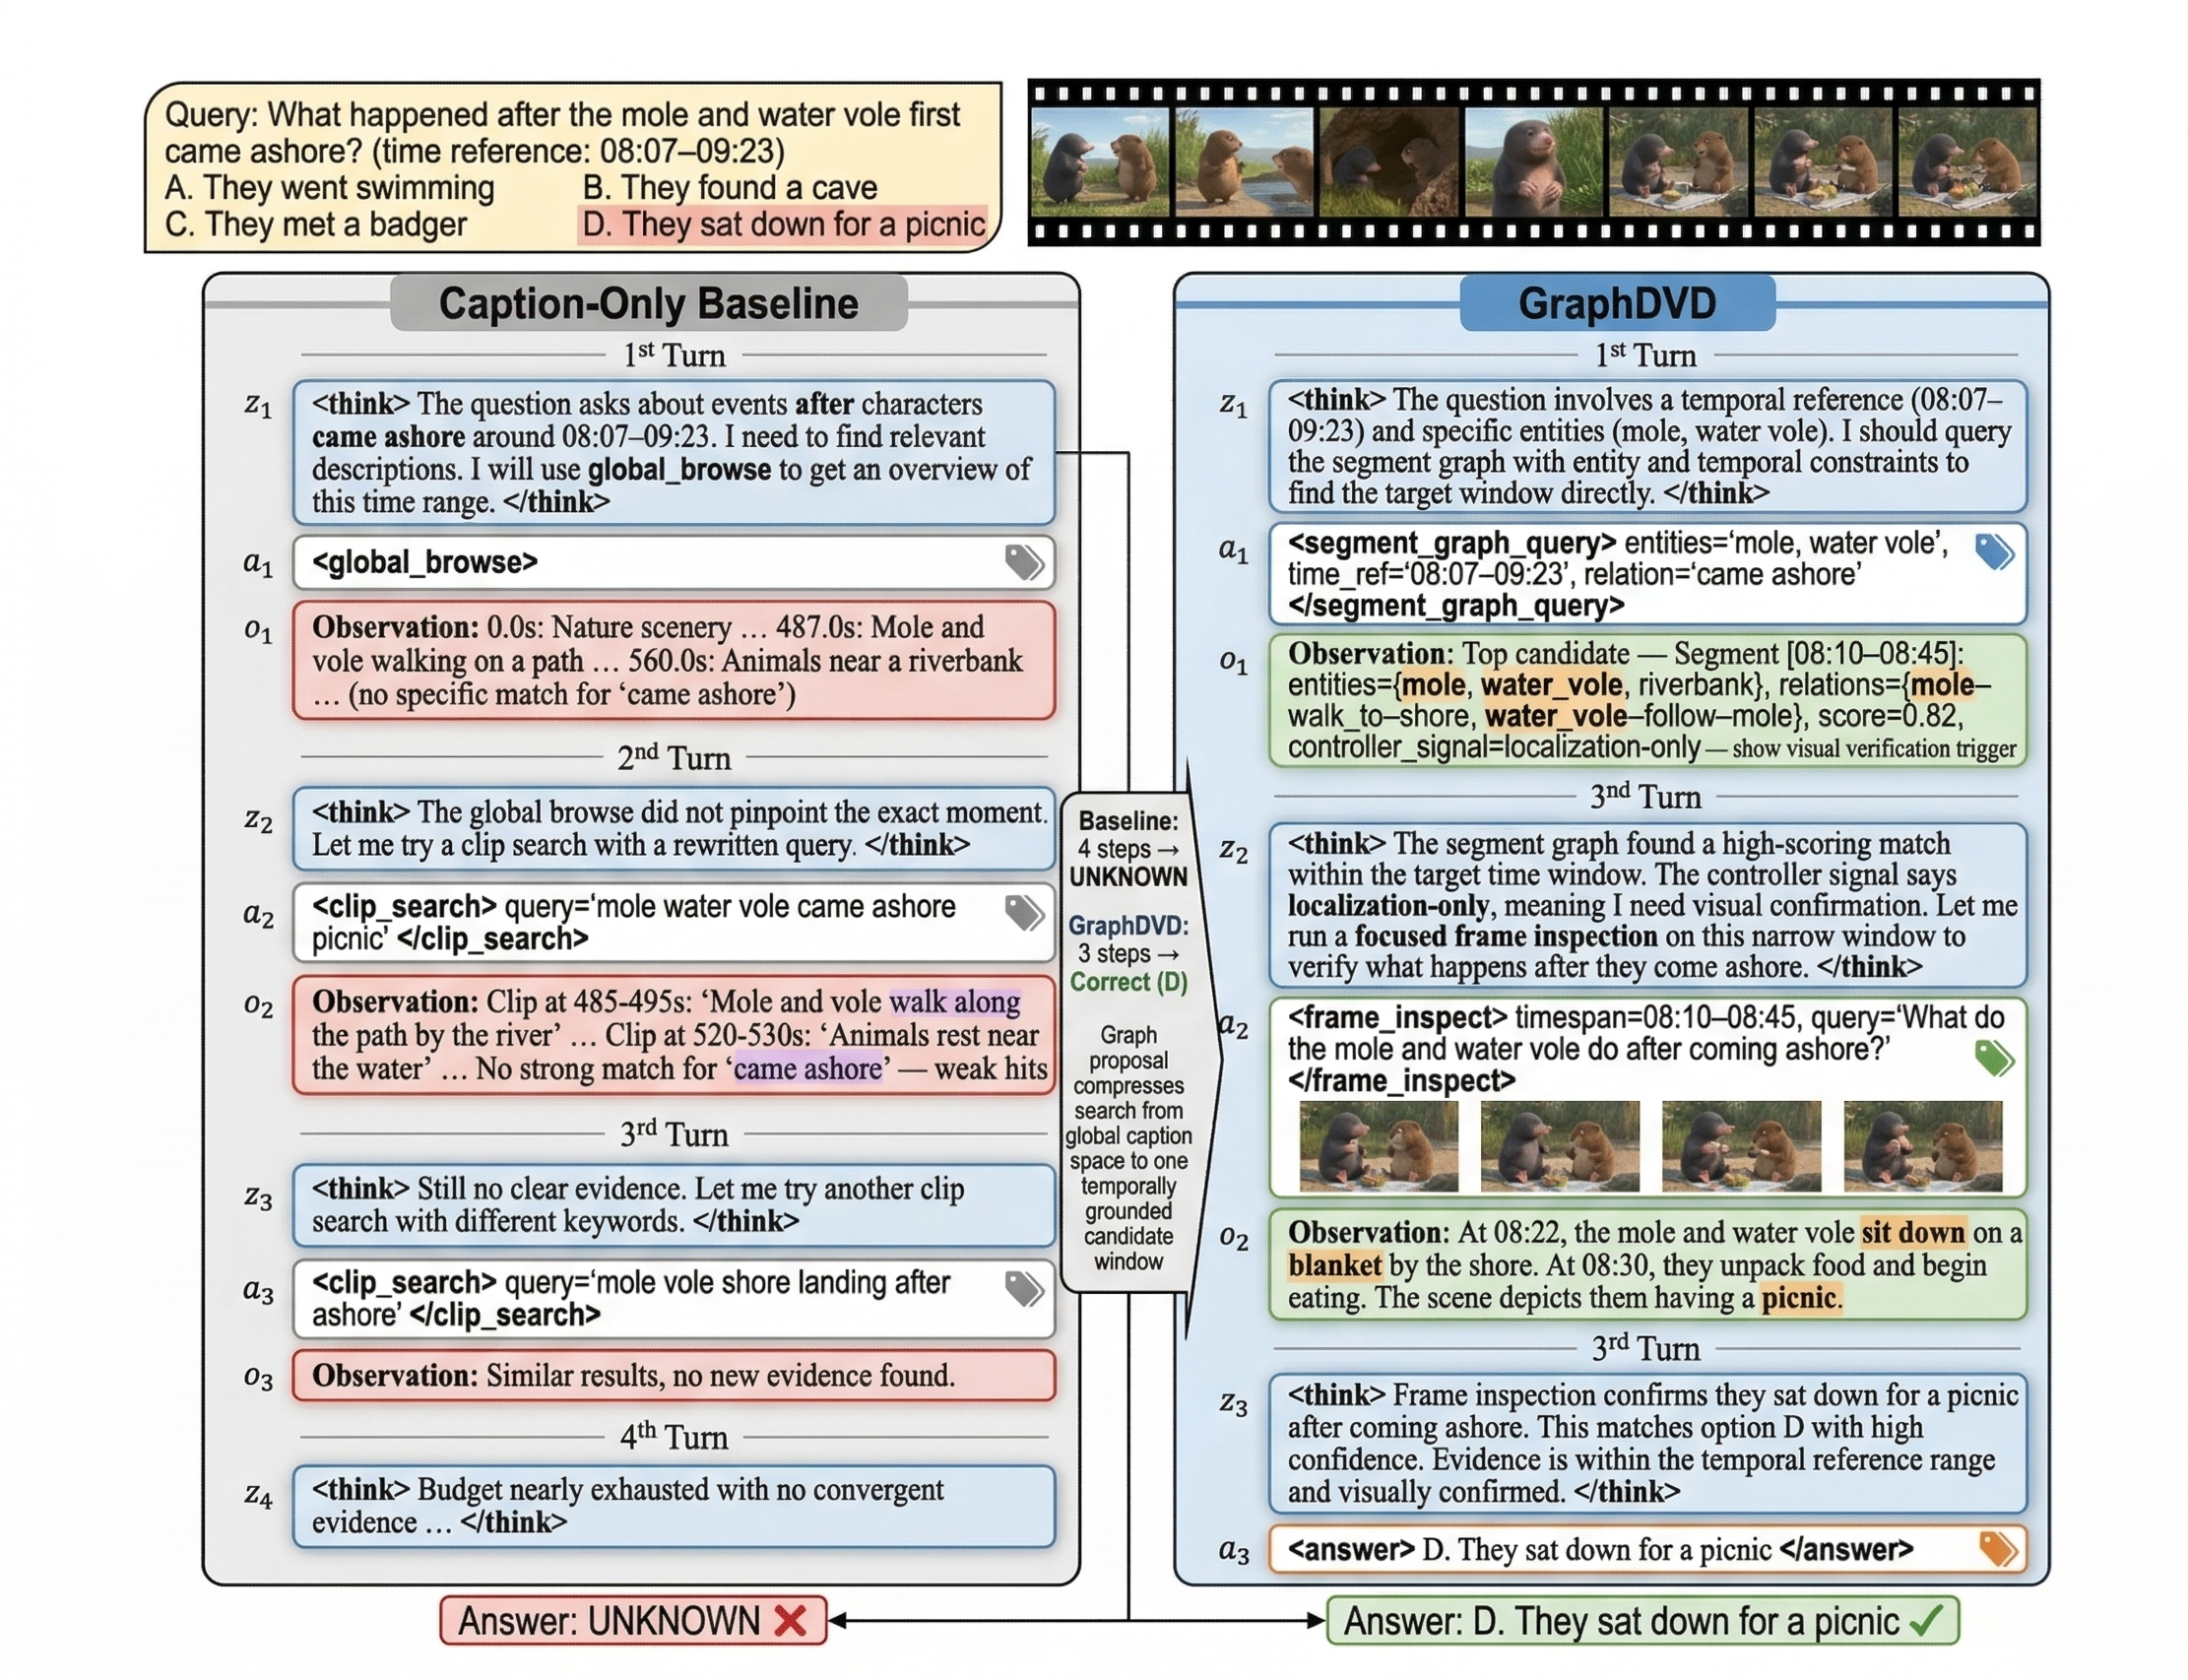
\includegraphics[width=\textwidth]{figures/Case.png}
  \caption{Trajectory comparison between the caption-only baseline and
           SGDAgent on three representative question types. Graph query
           tools (\textcolor{blue}{blue}) replace broad caption searches
           (\textcolor{gray}{gray}) and guide focused frame inspections
           (\textcolor{green!60!black}{green}) to narrow candidate
           windows, yielding shorter and more targeted trajectories. The
           rightmost case illustrates a failure mode where correct
           localization does not prevent an incorrect visual judgment.}
  \label{fig:trajectory}
\end{figure*}

\section{Conclusion}

This paper proposes SGDAgent for augmenting the caption database with a hierarchical scene graph index in long-form video question answering. The core conclusion is not that ``the graph module brings some additional improvement'' but a stronger search paradigm thesis: \textbf{SGDAgent converts open-ended caption search into graph-anchored candidate verification.}

This thesis uniformly explains the main method design and experimental results. First, it explains why the graph-augmented database is necessary: caption alone retains an overly large open search space, while graph alone is insufficient to cover open semantic descriptions, so both must complement each other. Second, it explains why SGDAgent can significantly reduce FTT: when search transforms from open-ended recall to candidate verification, the agent more easily forms stable trajectories and commits terminal judgments. Finally, it explains why accuracy improves: SGDAgent not only answers more questions but also achieves higher verification quality on already-answered samples.

From current results, SGDAgent's primary gains come from Stage~1 and Stage~2's local structured candidate discovery, while Stage~3 further supplements event-level candidate proposal, event chain modeling, and event-to-segment cascade. Future work can proceed along two directions: improving local visual verification reliability to reduce residual errors from ``FTT to wrong answer'' conversions, and enhancing the global event graph's event abstraction and chain retrieval capabilities for more stable long-range event reasoning.


%%
%% Acknowledgments
%%
\begin{acks}
% Hidden during anonymous review. Fill in after acceptance.
\end{acks}

%%
%% Bibliography
%%
\bibliographystyle{ACM-Reference-Format}
\bibliography{references}

\end{document}
